\chapter{Datasets}

This thesis is based on 5 different already existing datasets.
This chapter discusses these datasets based on different criteria:

\begin{description}
    \item[source:] reference of the owner of the dataset and brief description of the original purpose of the dataset. Importantly, this part also discusses the source of the annotation.
    \item[Patient sample:] statistics of the patients of whom medical images were collected such as age, gender and possible spine pathologies.
    \item[Technical information:] discusses the imaging technology, the image resolution and the spatial dimensions of the image. 
\end{description}

\section{Global overview of the different dataset}

\todo[inline]{Overview of the datasets gathered. MRI / CT, number of images, type of annotation + WHO performed the annotation? Was it a medical docter or one of the researchers.}



bla

\begin{SCtable}[\sidecaptionrelwidth][h]
 
    \begin{tabular}{ l l l l l} 
     \hline
     \hline
     Name & reference & imaging & Quantity & Annotation \\
          &           & technology & [images] & \\
     \hline 
    UWSpine & \cite{Glocker}  & \acrshort{ct} & 125 & point  \\ 
    xVertSeg & \cite{Ibragimov2014, Korez2015} & \acrshort{ct} & 15 & full \\
    UniSiegen  & \cite{Zukic2014} & \acrshort{mri} & 17 & full \\
    PLoS & \cite{Chu2015} & \acrshort{mri} & 23 & semantic \\
    MyoSegmenTUM & \cite{Burian2019} & \acrshort{mri} &  54 & full \\
     \hline
     \hline
    \end{tabular}
    \caption{List of dataset references. For more details on the data quantity, please consult chapter \ref{seg:datasetcomparison}. 
    Notably the fact that some images were taken from the same patient is important. This means the dataset is grouped. 
    The agreement with prof. T. Vrtovec regarding the xVertSeg dataset can be found in appendix \ref{seg:datasetagreement}.}

\end{SCtable}

\begin{SCtable}[\sidecaptionrelwidth][h]
 
    \begin{tabular}{ l l l l} 
     \hline
     \hline
     Name & X & Y & Z \\
     \hline 
    UWSpine & Left-right & Anteroposterior & Craniocaudal \\
    xVertSeg & Left-right & Anteroposterior & Craniocaudal \\
    UniSiegen  &  Anteroposterior & Craniocaudal & Left-right \\
    PLoS & Left-right & Anteroposterior & Craniocaudal$^\dagger$ \\
    MyoSegmenTUM &  Anteroposterior & Craniocaudal & Left-right \\
     \hline
     \hline
    \end{tabular}
    \caption{List of dataset references. For more details on the data quantity, please consult chapter \ref{seg:datasetcomparison}. 
    Notably the fact that some images were taken from the same patient is important. This means the dataset is grouped. 
    The agreement with prof. T. Vrtovec regarding the xVertSeg dataset can be found in appendix \ref{seg:datasetagreement}.
    $^\dagger$ The Craniocaudal axis in the PLoS dataset is inverted.}

\end{SCtable}

\section{Comparison of the different datasets\label{seg:datasetcomparison}}


\subsection{xVertSeg\label{sec:xVertSeg}}



The xVertSeg \cite{Ibragimov2012, xxx} was kindly made available by prof. T. Vrtovec (University of Ljubljana, Faculty of Electrical Engineering, Slovenia), see appendix \ref{seg:datasetagreement} for the agreement.
This dataset contains 25 \acrfull{ct} scans of the lumbar spine, of which 15 \acrshort{ct} scans are fully labeled.
Given the provided data, I can assume these 15 scans were collected from 15 different patients.

For each of these 15 scans, full instance segmenation masks for all 5 lumbar vertebrae are provided. The delineation was performed by a skilled professional.

Additionally, for each vertebra a fracture class and fracture grade is provided. 
Apart from vertebrae classified as \textit{normal}, the dataset contains \textit{mild}, \textit{moderate} and \textit{severe} cases of vertebrae fracture types \textit{wedge}, \textit{crush} and \textit{biconcavity}.
\marginpar{
        % This file was created by tikzplotlib v0.9.8.
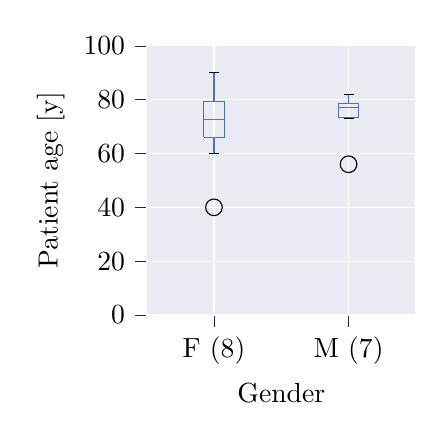
\begin{tikzpicture}

\definecolor{color0}{rgb}{0.917647058823529,0.917647058823529,0.949019607843137}
\definecolor{color1}{rgb}{0.298039215686275,0.447058823529412,0.690196078431373}
\definecolor{color2}{rgb}{0.768627450980392,0.305882352941176,0.32156862745098}

\begin{axis}[
axis background/.style={fill=color0},
axis line style={white},
height=5cm,
tick align=outside,
tick pos=left,
width=5cm,
x grid style={white},
xlabel={Gender},
xmajorgrids,
xmin=0.5, xmax=2.5,
xtick style={color=white!15!black},
xtick={1,2},
xticklabels={F (8),M (7)},
y grid style={white},
ylabel={Patient age [y]},
ymajorgrids,
ymin=0, ymax=100,
ytick style={color=white!15!black}
]
\addplot [color1, opacity=1]
table {%
0.925 66
1.075 66
1.075 79.25
0.925 79.25
0.925 66
};
\addplot [color1, opacity=1]
table {%
1 66
1 60
};
\addplot [color1, opacity=1]
table {%
1 79.25
1 90
};
\addplot [black, opacity=1]
table {%
0.9625 60
1.0375 60
};
\addplot [black, opacity=1]
table {%
0.9625 90
1.0375 90
};
\addplot [black, mark=o, mark size=3, mark options={solid,fill opacity=0}, only marks]
table {%
1 40
};
\addplot [color1, opacity=1]
table {%
1.925 73.5
2.075 73.5
2.075 78.5
1.925 78.5
1.925 73.5
};
\addplot [color1, opacity=1]
table {%
2 73.5
2 73
};
\addplot [color1, opacity=1]
table {%
2 78.5
2 82
};
\addplot [black, opacity=1]
table {%
1.9625 73
2.0375 73
};
\addplot [black, opacity=1]
table {%
1.9625 82
2.0375 82
};
\addplot [black, mark=o, mark size=3, mark options={solid,fill opacity=0}, only marks]
table {%
2 56
};
\addplot [color2, opacity=1]
table {%
0.925 72.5
1.075 72.5
};
\addplot [color2, opacity=1]
table {%
1.925 77
2.075 77
};
\end{axis}

\end{tikzpicture}

        \captionof{figure}{xVertSeg patients age distribution}
        \label{fig:xVertSeg_Age}
    }

\subsubsection{Original Objective of the Dataset}

The objective of the \textit{xVertSeg challenge}\footnote{see \url{http://lit.fe.uni-lj.si/xVertSeg/database.php}} (2015) was organized by the University of Ljubljana.
Based on the 15 provided scans with corresponding masks, the participans were required to construct a model to make predictions on the test set of 10 unlabelled scans.

The challenge consisted of two tasks:
\begin{enumerate}
    \item Segmentation of the lumbar vertebrae. For each scan in the test set, the segmentation masks of the lumbar vertebrae were requested.
    \item Fracture classification on the segmented vertebrae, consisting of morphological grade and fracture classification.
\end{enumerate}

\subsubsection{Patient statistics}

The patients in the xVertSeg dataset train set consist of 8 females and 7 males.
The age of these patients is slightly higher than for the other datasets.
The average patient in this dataset is 71 years old.
A box plot of the age distribution between genders is shown in figure \ref{fig:xVertSeg_Age}. 

\begin{SCtable}[\sidecaptionrelwidth][h]
    \centering
        \begin{tabular}{lrrrrrr}
\toprule
{} &  L1 &  L2 &  L3 &  L4 &  L5 &  Total \\
\midrule
biconcave &   6 &   7 &   8 &   4 &   2 &     27 \\
normal    &   5 &   6 &   4 &   4 &   7 &     26 \\
wedge     &   3 &   2 &   2 &   3 &   2 &     12 \\
crush     &   1 &   0 &   1 &   4 &   4 &     10 \\
\bottomrule
\end{tabular}

        \caption{Every patient in the xVertSeg dataset suffers from at least one spine pathology.
        Most of these pathologies are identified as \textit{mild}.
        This table counts the spine pathologies and normal vertebrae observed over all 15 patients in the xVertSeg dataset.}   
\end{SCtable}

\subsubsection{Technical information}

The xVertSeg dataset contains 15 \acrshort{ct} annotated scans. 
This dataset is very interesting due to the high quality and high resolution of the images.
On figure \ref{fig:xVertSeg_image002}, two slices of the same patient (002) are represented.
The slices show the complete, uncropped sections of the torso and abdominal region of the patient. 
There is no \acrshort{roi} cropping.

\begin{SCfigure}[][htb]
    \centering
    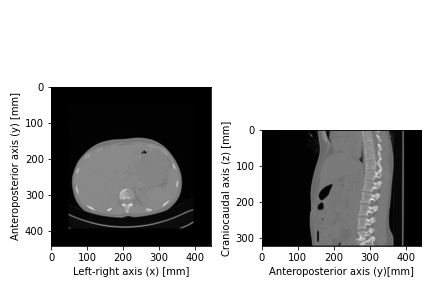
\includegraphics[width=.95\textwidth]{automated_graphs/xVertSeg_image002.png}
    \caption{xVertSeg scan \textit{image002}. \label{fig:xVertSeg_image002}}
\end{SCfigure}

The distribution of the scan dimensions is shown in figure \ref{fig:AllDataset_dims}. This also illustrates the \textit{xVertSeg} dataset consists of large, high resolution images.
Mind that during pre-processing the scans are resampled on a $1mm \times 1mm \times 1mm$ grid.


\subsection{UniSiegen dataset\label{sec:DataUSiegen}}

This dataset is made available in 2014 by the University of Siegen, Germany.
Dr D. Zukic \cite{Zukic2014} constructed it as part of his PhD project.

\marginpar{
        % This file was created by tikzplotlib v0.9.8.
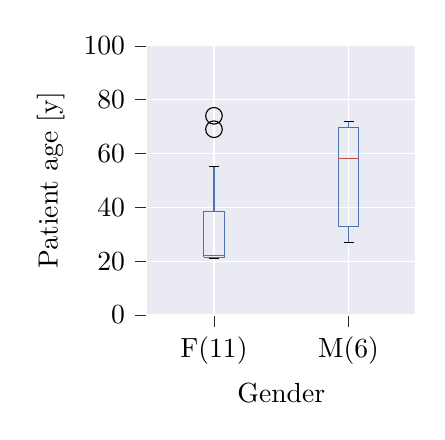
\begin{tikzpicture}

\definecolor{color0}{rgb}{0.917647058823529,0.917647058823529,0.949019607843137}
\definecolor{color1}{rgb}{0.298039215686275,0.447058823529412,0.690196078431373}
\definecolor{color2}{rgb}{0.768627450980392,0.305882352941176,0.32156862745098}

\begin{axis}[
axis background/.style={fill=color0},
axis line style={white},
height=5cm,
tick align=outside,
tick pos=left,
width=5cm,
x grid style={white},
xlabel={Gender},
xmajorgrids,
xmin=0.5, xmax=2.5,
xtick style={color=white!15!black},
xtick={1,2},
xticklabels={F(11),M(6)},
y grid style={white},
ylabel={Patient age [y]},
ymajorgrids,
ymin=0, ymax=100,
ytick style={color=white!15!black}
]
\addplot [color1, opacity=1]
table {%
0.925 21.5
1.075 21.5
1.075 38.5
0.925 38.5
0.925 21.5
};
\addplot [color1, opacity=1]
table {%
1 21.5
1 21
};
\addplot [color1, opacity=1]
table {%
1 38.5
1 55
};
\addplot [black, opacity=1]
table {%
0.9625 21
1.0375 21
};
\addplot [black, opacity=1]
table {%
0.9625 55
1.0375 55
};
\addplot [black, mark=o, mark size=3, mark options={solid,fill opacity=0}, only marks]
table {%
1 74
1 69
};
\addplot [color1, opacity=1]
table {%
1.925 33
2.075 33
2.075 69.5
1.925 69.5
1.925 33
};
\addplot [color1, opacity=1]
table {%
2 33
2 27
};
\addplot [color1, opacity=1]
table {%
2 69.5
2 72
};
\addplot [black, opacity=1]
table {%
1.9625 27
2.0375 27
};
\addplot [black, opacity=1]
table {%
1.9625 72
2.0375 72
};
\addplot [color2, opacity=1]
table {%
0.925 22
1.075 22
};
\addplot [color2, opacity=1]
table {%
1.925 58
2.075 58
};
\end{axis}

\end{tikzpicture}

        \captionof{figure}{USiegen patients age distribution}
        \label{fig:USiegen_Age}
    }

This dataset contains 26 \acrshort{mri} scans of 17 different patients\footnote{This is not clearly stated, but can be inferred from the metadata.}. 
The fact that scans of the same patient are correlated will be taken into account in the train, validation and test split.
For more details on this split, see section \ref{sec:trainValTestSplit} on page \pageref{sec:trainValTestSplit}.

\subsubsection{Original Objective of the Dataset}

This dataset was collected from several hospitals (Sarajevo, Marburg, Brisbane, Schwabach, Bad Wildungen \& Prague). The MRI scanner settings were varied between the scans (T1, T2, TIRM).
The PhD project objective was to build a segmentation model to automate the segmentation of the lumbar vertebrae in the \acrshort{mri} scans to facilitate the diagnosis of several spine pathologies 
such as scoliosis, spondylolisthesis \footnote{Spondylolisthesis is the displacement of one spinal vertebra compared to another.} and vertebral fractures.
The final model developed by dr. D. Zukic consisted of a Viola-Jones detector for detection and vertebral body size approximation.
The average Dice score compared to the manual reference was reported to be 79.3\%.

\subsubsection{Patient statistics}

In \cite{Zukic2014}, it is not entirely made clear which scans are taken from the same patient.
It is made clear, however that the 26 scans were not obtained from 26 patients.
The information was inferred from the naming of the scans and the provided gender en age information\footnote{
    Wrongfully assuming two scans come from the same patient does not cause data leakage.
}.

Figure \ref{fig:USiegen_Age} illustrates that the USiegen dataset contains almost double the number of female patients compared to male patients.
These patients are relatively young compared to the patients in the \textit{xVertSeg} dataset.

Only three of the patients in this dataset were categorized as having no spinal pathologies.

\subsubsection{Technical information}

Several \acrlong{mri} techniques were used to obtain the dataset: T1, T2 \& TIRM.
I do not take into account this factor in the model development or the dataset split.

The volumes in the USiegen dataset are strongly cropped. 
Both in the anteroposterior and the craniocaudal direction, the volumes are on average 370 mm.
In the left-right direction, however, the volumes have been cropped severely. The volumes are, on average, only 68 mm wide.
The images have been cropped to only include the \acrshort{roi}.
Along this left-right dimension, the voxel spacing is large. 

\begin{SCfigure}[][htb]
    \centering
    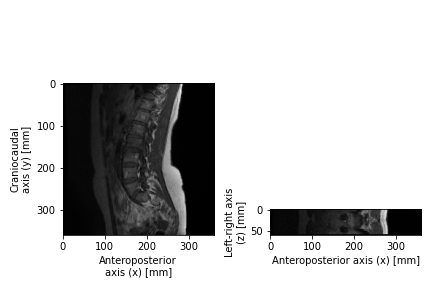
\includegraphics[width=.95\textwidth]{automated_graphs/USiegen_Aka3.png}
    \caption{USiegen dataset scan \textit{Aka3}. \label{fig:USiegen_Aka3}. It is immediately clear the USiegen volumes are cropped differently than the xVertSeg volumes.
    In the craniocaudal direction, both sacrum and coccyx are visible. Along the left-righ axis, the volumes have been cropped severely.}
\end{SCfigure}

The original scans in the \textit{USiegen} dataset were cropped in the \textit{left-right} direction. 
Although the scan resolution is relatively high in the Sagittal planes, the slice spacing along the left-right axis is coarser (see figure \ref{fig:AllDataset_dims}).  
\subsection{PLoS Dataset}

The \textit{PLoS} dataset was compiled for \cite{Chu2015} in 2015 by dr. C. Chu, University of Bern, Bern, Switzerland and made publically available \footnote{See : \url{ http://doi.org/10.5281/zenodo.22304 }} .
It consists of 23 T2-weighted spine \acrshort{mri} scans. 
Contrary to other datasets, the segmenation labels in this dataset do not provide information to destinguish the individual vertebrae from each other.

\subsubsection{Original Objective of the Dataset}

In \cite{Chu2015} the development of a random forest regression approach for spine vertebrae segmenation and classificiation is described.
The results of several random forest regressors and classifiers is unified with a voting mechanism.
This approach obtains a mean Dice metric score of 88.7\%.

\subsubsection{Patient statistics}

Due to the anomimization process, the \textit{PLoS} dataset does not contain patient information.
This means that it is not possible to produce any statistics regarding patient age or gender.

\subsubsection{Technical information}

As is indicated in figure \ref{fig:AllDataset_dims}, and in figure \ref{fig:PLoS_img02}, the PLoS image volumes are cropped in the left-right direction.
The volumes are consistently $381mm \times 381 mm \times 78 mm$, where the shortest dimension is in the left-right direction.

\begin{SCfigure}[][htb]
    \centering
    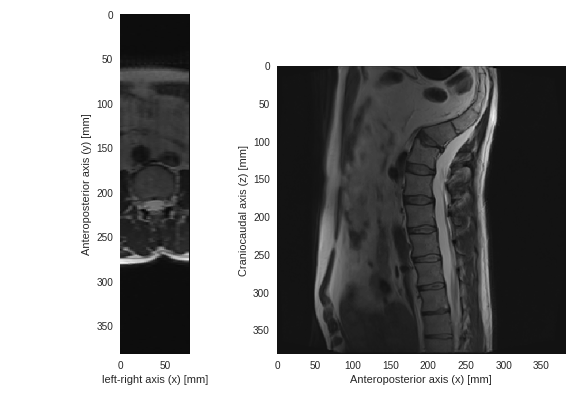
\includegraphics[width=.95\textwidth]{automated_graphs/PLoS_img02.png}
    \caption{
        PLoS dataset scan \textit{img02}. \label{fig:PLoS_img02}. The craniocaudal direction is cropped in a way comparable to the volumes in the USiegen dataset, but, the direction of this axis is inverted.
        The left-right axis is cropped similar to the USiegen data volumes.
    }
\end{SCfigure}
\subsection{MyoSegmenTUM datset}

This dataset is made available by S. Schläger from the Technische Universität München via the \acrfull{osf} \footnote{see \url{ https://osf.io/3j54b/?view_only=f5089274d4a449cda2fef1d2df0ecc56 }}.
It was constructed for the MyoSegmenTUM project \cite{Burian2019}.
It consists of 54 collections of \acrshort{mri} scans of the spine.
In this work, only the T2 weighted \acrlong{mri} scans are used.
The dataset also contains volumes with enhanced fat tissue response. Since the objective of this work is related to bone tissue rather than fat tissue, these volumes were not used.
Neither was the segmentation masks for the different dorsal muscles, which are also present in this dataset.

\subsubsection{Original Objective of the Dataset}

The MyoSegmenTUM Spine dataset is compiled as a reference dataset for developing segmentation algorithms of the lumbar spine vertebral bodies and muscle groups.
Information about this project can be found in \cite{Burian2019}.

\subsubsection{Patient statistics}

In figure \ref{fig:OSF_ageboxplot}, the age distribution of the patients in the MyoSegmenTUM dataset is shown.
There are more women (39) included in this dataset than men (15).
The male patients in this dataset are, on average, clearly younger than the female patients.

\marginpar{
        % This file was created by tikzplotlib v0.9.8.
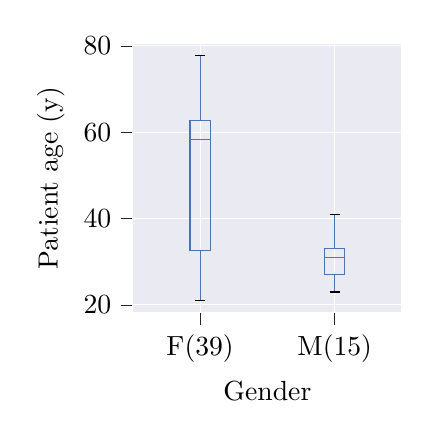
\begin{tikzpicture}

\definecolor{color0}{rgb}{0.917647058823529,0.917647058823529,0.949019607843137}
\definecolor{color1}{rgb}{0.298039215686275,0.447058823529412,0.690196078431373}
\definecolor{color2}{rgb}{0.768627450980392,0.305882352941176,0.32156862745098}

\begin{axis}[
axis background/.style={fill=color0},
axis line style={white},
height=5cm,
tick align=outside,
tick pos=left,
width=5cm,
x grid style={white},
xlabel={Gender},
xmajorgrids,
xmin=0.5, xmax=2.5,
xtick style={color=white!15!black},
xtick={1,2},
xticklabels={F(39),M(15)},
y grid style={white},
ylabel={Patient age (y)},
ymajorgrids,
ymin=18.1666324435318, ymax=80.5007186858316,
ytick style={color=white!15!black}
]
\addplot [color1, opacity=1]
table {%
0.925 32.5
1.075 32.5
1.075 62.7652292950034
0.925 62.7652292950034
0.925 32.5
};
\addplot [color1, opacity=1]
table {%
1 32.5
1 21
};
\addplot [color1, opacity=1]
table {%
1 62.7652292950034
1 77.6673511293635
};
\addplot [black, opacity=1]
table {%
0.9625 21
1.0375 21
};
\addplot [black, opacity=1]
table {%
0.9625 77.6673511293635
1.0375 77.6673511293635
};
\addplot [color1, opacity=1]
table {%
1.925 27
2.075 27
2.075 33
1.925 33
1.925 27
};
\addplot [color1, opacity=1]
table {%
2 27
2 23
};
\addplot [color1, opacity=1]
table {%
2 33
2 41
};
\addplot [black, opacity=1]
table {%
1.9625 23
2.0375 23
};
\addplot [black, opacity=1]
table {%
1.9625 41
2.0375 41
};
\addplot [color2, opacity=1]
table {%
0.925 58.2888432580424
1.075 58.2888432580424
};
\addplot [color2, opacity=1]
table {%
1.925 31
2.075 31
};
\end{axis}

\end{tikzpicture}

        \captionof{figure}{Distribution of patient age in the dataset from the MyoSegmenTUM project.}
        \label{fig:OSF_ageboxplot}
    }


\subsubsection{Technical information}

As shown in figure \ref{fig:OSF_02}, coupes from the second volume of the MyoSegmenTUM dataset are shown.
As is also indicated in figure \ref{fig:AllDataset_dims}, the dimensions of the MyoSegmenTUM volumes is consistent $220 mm \times 220 mm \times 80 mm$, where the shortest dimension is the cropped left-right axis.
There are only three volumes that deviate slightly from this.

\begin{SCfigure}[][htb]
    \centering
    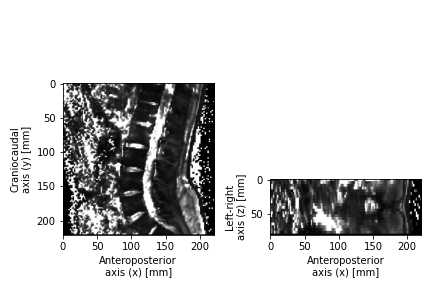
\includegraphics[width=.95\textwidth]{automated_graphs/OSF_02.png}
    \caption{MyoSegmenTUM dataset scan \textit{02}. 
    The volumes are cropped in the left-right direction. 
    \label{fig:OSF_02}}
\end{SCfigure}

\textbf{Remark:} For three volumes (nr 33, 53 and 54) for which the dimension of the image volume and the label mask do not correspond. 
It is not clear how these masks should be used. 
These volumes were discarded, bringing the final number of volumes used from the MyoSegmenTUM dataset to 51.
\subsection{UWSpine dataset}
 
This dataset is made available by the Department of Radiology of the University of Washington\footnote{Creative Commons Attribution-NonCommercial-NoDerivatives 4.0 International License, dataset available at \url{
      https://biomedia.doc.ic.ac.uk/data/spine/  
    }}.
It has been constructed by dr. Glocker and team \cite{Glocker2012,Glocker2013} (Microsoft research) in 2012.
For each scan, manual annotations of vertebrae centroids are provided.
This dataset contains 242 \acrshort{ct} scans of 150 different patients.
This dataset does not contain full mask labels, only centroid point annotations.
To investigate the relative performance of a weakly supervised model compared to the performance of a fully supervised model, both will be trained on the same dataset\footnote{The modelling concept is further discussed in chapter \ref{sec:model_concept}.}.
Furthermore, the evaluation of the models is based on the full annotations.
Thus, the UWSpine dataset will not be used for model training.
It will only be used for visual evaluation of the model on a completely new dataset\footnote{The UWSpine dataset is \textit{completely} new in the sense that no samples from this dataset (this \textit{population}, so to speak) are present in the train or validation set.
For the \textit{normal} test set, other samples from the same datasets where present in the train and validation sets.}.


\subsubsection{Original Objective of the Dataset}

In \cite{Glocker2012,Glocker2013} the development of a model based on regression forests and a \acrfull{hmm} for vertebra localisation without needing strong assumptions on what part of the spine is visible.

\subsubsection{Patient statistics}


Figure \ref{fig:UW_ageboxplot} illustrated that the patients in the \textit{UWSpine} dataset are relatively varied in age.
Of most patients in the dataset, multiple scan images are available.
The highest number of scans taken from a single patient is 5.

\subsubsection{Technical information}

Only point annotations are available for the \textit{UWSpine} dataset. 
This means this dataset can only be used for weakly supervised model training.

The scans in the \textit{UWSpine} dataset are strongly cropped around the spine, both in the left-right direction and the anteroposterior direction.

\begin{SCfigure}[][htb]
    \centering
    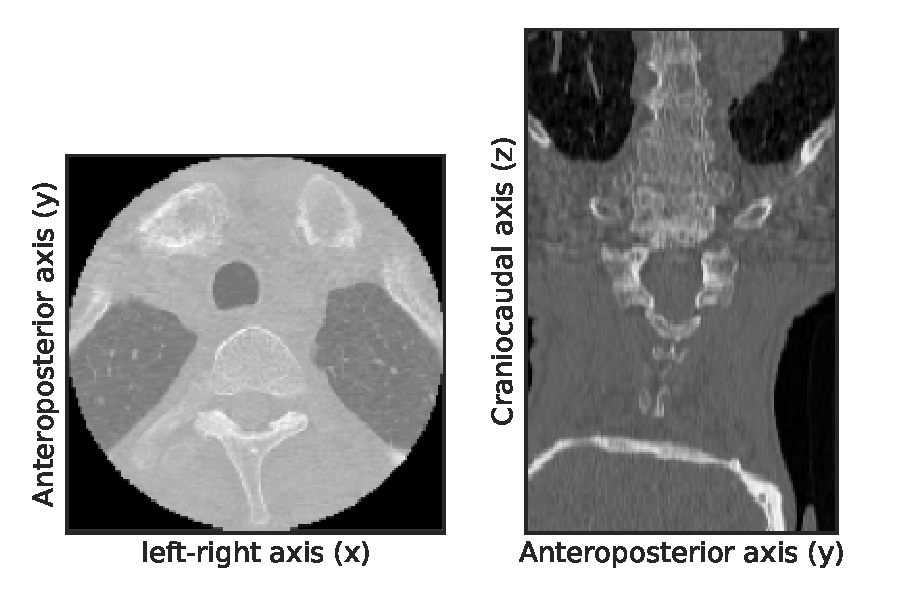
\includegraphics[width=.95\textwidth]{automated_graphs/UW_4564688.pdf}
    \caption{University of Washington dataset, scan \textit{4564688}. \label{fig:UW_4564688}}
\end{SCfigure}

\marginpar{
        % This file was created by tikzplotlib v0.9.8.
\begin{tikzpicture}

\definecolor{color0}{rgb}{0.917647058823529,0.917647058823529,0.949019607843137}
\definecolor{color1}{rgb}{0.298039215686275,0.447058823529412,0.690196078431373}
\definecolor{color2}{rgb}{0.768627450980392,0.305882352941176,0.32156862745098}

\begin{axis}[
axis background/.style={fill=color0},
axis line style={white},
tick align=outside,
tick pos=left,
x grid style={white},
xlabel={Gender},
xmajorgrids,
xmin=0.5, xmax=2.5,
xtick style={color=white!15!black},
xtick={1,2},
xticklabels={Female (54 patients),Male (71 patients)},
y grid style={white},
ylabel={Patient age (y)},
ymajorgrids,
ymin=11.05, ymax=97.95,
ytick style={color=white!15!black}
]
\addplot [color1, opacity=1]
table {%
0.925 42.75
1.075 42.75
1.075 64.75
0.925 64.75
0.925 42.75
};
\addplot [color1, opacity=1]
table {%
1 42.75
1 15
};
\addplot [color1, opacity=1]
table {%
1 64.75
1 94
};
\addplot [black, opacity=1]
table {%
0.9625 15
1.0375 15
};
\addplot [black, opacity=1]
table {%
0.9625 94
1.0375 94
};
\addplot [color1, opacity=1]
table {%
1.925 41.5
2.075 41.5
2.075 65.5
1.925 65.5
1.925 41.5
};
\addplot [color1, opacity=1]
table {%
2 41.5
2 15
};
\addplot [color1, opacity=1]
table {%
2 65.5
2 90
};
\addplot [black, opacity=1]
table {%
1.9625 15
2.0375 15
};
\addplot [black, opacity=1]
table {%
1.9625 90
2.0375 90
};
\addplot [color2, opacity=1]
table {%
0.925 54
1.075 54
};
\addplot [color2, opacity=1]
table {%
1.925 54
2.075 54
};
\end{axis}

\draw ({$(current bounding box.south west)!0.5!(current bounding box.south east)$}|-{$(current bounding box.south west)!0.98!(current bounding box.north west)$}) node[
  scale=0.6,
  anchor=north,
  text=white!15!black,
  rotate=0.0,
  align=center
]{OSF dataset
age distribution};
\end{tikzpicture}

        \captionof{figure}{Distribution of patient age in the dataset from Washington University.}
        \label{fig:UW_ageboxplot}
    }